\section{Library Structures}
\begin{frame}
  \begin{center}
    {\large Lecture 02 -- Data Structures\\Part III -- Data Structures from Libraries}\\
  \end{center}
\end{frame}

\begin{frame}
  \frametitle{Learn your data structure libraries}

  \begin{itemize}
    \item The standard C++ library (STL) implements many useful data structures;
    \item By using data structures from the STL, you make your program simpler and avoids bugs;
      \bigskip

    \item In this section, we will review some of the data structures used most often.
    \item We will focus on usage, rather than theory.
      \bigskip

    \item For more information about how these data structures work, we recomment the the website \url{https://visualgo.net/};
  \end{itemize}

\end{frame}

%%%%%%%%%%%%%%%%%%%%%%%%%%%%%%%%%%%%%%%%%%%%%%%%%%%%%%%%%
\subsection{Deque, Queue, Stack}

%% TODO: Add Motivating Problem For Queue
\begin{frame}
  \frametitle{Vector variations: Deque, Queue, Stack}

  While the \emph{vector} is a general and useful data structure, for some applications you will want special access to the {\bf start} and {\bf end} of a vector. \bigskip

  \begin{itemize}
    \item \structure{stack}: \emph{pop} and \emph{push} from the front of the vector;
    \bigskip

    \item \structure{queue}: \emph{pop} from the back, \emph{push} from the front;
    \bigskip

    \item \structure{deque}: \emph{pop\_front, push\_front, pop\_back, push\_back};
  \end{itemize}
  \bigskip

  \begin{block}{Behind C++}
    Actually, \emph{Queue} and \emph{Stack} are high level constructs,
    \structure{List} or \structure{Deque} are used to implement them.
  \end{block}
\end{frame}

\begin{frame}[fragile]
  \frametitle{Queue and Stacks}

  \begin{block}{}
    Queues and Stacks are useful to simplify common cases of vectors
  \end{block}

  Stack Example: Test if a set of parenthesis is balanced.
{\small
\begin{verbatim}
#include <stack>
stack<char> s;
char c;

while(cin >> c) {
  if (c == '(') s.push(c);
  else {
    if (s.size() == 0) { s.push('*'); break; }
    s.pop();
  }
}
cout << (s.size() == 0 ? "balanced" : "unbalanced");
\end{verbatim}}
\end{frame}


\subsection{Maps and Sets}

\begin{frame}{Maps and Sets}{Problem Example: CD -- 11849}

  Jack and Jill are comparing their CD collections. The problem wants to know: How many CDs are in the both collections?\bigskip

  \begin{block}{}
    {\bf Input:}
    \begin{itemize}
    \item Jack CD collection: List of $10^6$ CD IDs
    \item Jill CD collection: List of $10^6$ CD IDs
    \item Each CD ID is an integer from 1 to $10^9$
    \end{itemize}

    {\bf Output:}
    \begin{itemize}
    \item Number of CD IDs that appear in both collections.
    \end{itemize}

  \end{block}
  \bigskip

  Easy problem, right?
\end{frame}

\begin{frame}{Maps and Sets}{Problem Example: CD -- 11849}
  Naive Solution:
  \bigskip

  \begin{enumerate}
  \item Store all IDs in collection 1 in a Vector \hfill (n steps)
  \item Sort the Vector \hfill (nlogn steps)
  \item For each ID in collection 2, use Binary Search to find it in Vector 1\\
  \hfill (nlogn steps)
  \end{enumerate}

  Total Cost: $n + n\text{log}n + n\text{log}n$
  \vspace{2cm}

  \begin{block}{}
  Unfortunately, this is not fast enough for the time limit of this problem. Using the right data structure, you can reduce the time cost to $n+\log n$.
  \end{block}
\end{frame}

\begin{frame}[fragile]{Solving CD with a map data structure}{Approximate Solution}

  The STL provides {\bf set}, which is a data structure that uses balanced search trees to allow finding items in $\log n$

{\smaller
  \begin{block}{}
\begin{verbatim}
#include <iostream>
#include <set>
using namespace std;

int main() {
  int N, M, num; cin >> N >> M;
  set<int> first;
  while (N--) { cin >> num; first.insert(num); }
  int count = 0;
  for (int i = 0; i < M; i++) {
    cin >> num;
    if (first.find(num) != first.end()) ++count; }
  cout << count << '\n';
}
\end{verbatim}
\end{block}}
\end{frame}



\subsection{Balanced Search Trees}

\begin{frame}
  \frametitle{Balanced Search Trees}
  \begin{center}
    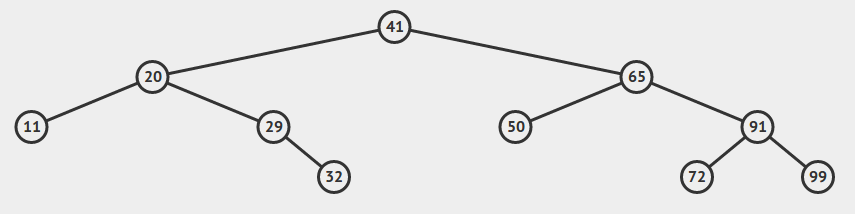
\includegraphics[width=0.8\textwidth]{img/BST}
  \end{center}
  \begin{itemize}
  \item \emph{Search Trees} Keep items in an ordered relationship.
  \item For example: Left children always have smaller values, Right
    children always have larger values;
  \item Insertion/Search/Deletion in a tree costs $O(h)$, where $h$ is
    the height of the tree;
  \item For a tree with $n$ elements, the \structure{minimum} height
    is $\text{log}n$
  \item For a balanced tree, the \structure{maximum} height is also
    $\text{log}n$
  \item How to keep the tree balanced?
  \end{itemize}
\end{frame}

\begin{frame}
  \frametitle{Balanced Search Trees}
  \framesubtitle{How to keep the tree balanced?}

  There are many Tree implementations/algorithms for keeping an BST
  balanced, and minimizing the tree height efficiently:
  \begin{itemize}
  \item AVL Tree (Adelson-Velskii-Landis);
  \item Red-Black Tree;
  \item B-Tree;
  \item Splay Tree;
  \end{itemize}
  \bigskip

  However, in for short programs (such as programming challenges)
  implementing these trees from scratch is a good way to create {\bf bugs}.
  \bigskip

  Luckly, most standard libraries include some implementation of BST.
\end{frame}

\begin{frame}
  \frametitle{ABLs in C++: Map and Set}

  \begin{itemize}
  \item In C++, the \emph{Map} and \emph{Set} classes are implemented
    using BSTs
  \item \emph{Map} Accept Key-value pairs;
  \item \emph{Set} Accepts only Keys;
  \end{itemize}

\end{frame}

\begin{frame}[fragile]
  \frametitle{Using Map in C++}
  {\small
  \begin{block}{}
\begin{verbatim}
#include <map>
map<string, int> ages; ages.clear();
ages["john"] = 40;
ages["billy"] = 39;
ages["andy"] = 29;
ages["steven"] = 42;
ages["felix"] = 33;
  // What is the age of andy?
map<string, int>::iterator it = ages.find("andy");
cout << it->second << endl;
  // Which names are between "f" and "m" ??
for (map<string, int>::iterator it =
     age.lower_bound("f");              // finds felix
     it != age.upper_bound("m"); it++)  // finds johm
        cout << " " << ((string)it->first).c_str();
\end{verbatim}
\end{block}}
\end{frame}

%% Already used this code in an earlier slide
% \begin{frame}[fragile]
%   \frametitle{Using Set in C++}
%   {\small
% \begin{verbatim}
% #include <set>
% set<int> CDs;
% CDs.clear();
%
% // Adding some values
% CDs.insert(1000); CDs.insert(999); CDs.insert(1337);
% CDs.insert(1313); CDs.insert(100020);
%
% // Testing if a particular value exists (O(logn))
% set<int>::iterator f = used_values.find(79);
% if (f == used_values.end())
%   cout << "not found!\n";
% else
%   cout << *f;    // Index!
% \end{verbatim}}
% \end{frame}

\subsection{Hash Tables}
\begin{frame}[fragile]
  \frametitle{Hash Tables}

  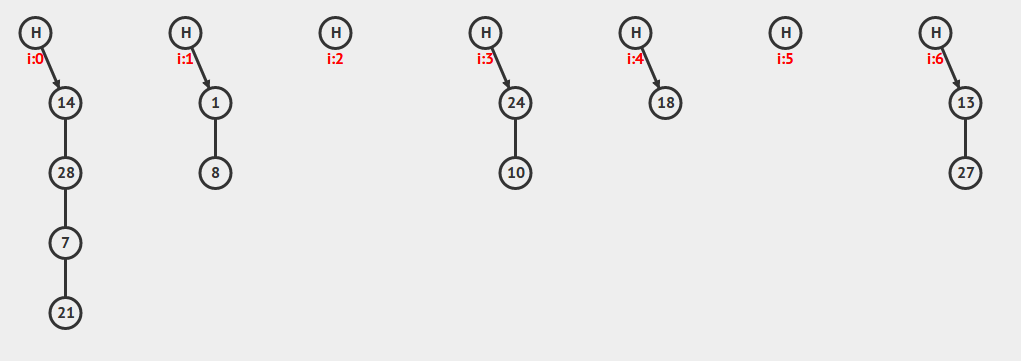
\includegraphics[width=0.95\textwidth]{img/hash}

  \begin{itemize}
  \item Insertion and Search: \structure{O(1)} -- \alert{Slow iteration};
  \item C++ library: \emph{std::unordered\_map};
  \item \structure{Hash} parameter -- Defines Collision results.
  \item Learn more about hash tables here: \url{https://visualgo.net/ja/hashtable}
  \end{itemize}
\end{frame}
